\section{Les rôles de \textbf{IA} dans la médecine}
\subsection{\mybox Introduction}
\subsection{\mybox Les rôles de \textbf{IA} dans la médecine}

\begin{frame}{Introduction}
    \begin{enumerate}[<+-|alert@+>]
        \myitem L'IA, par les algorithmes, aide donc principalement à l'élaboration de
                diagnostics.
        \myitem En effet, la machine prescrit le même diagnostic que les
                médecins dans 99\% des cas, et dans 30\% des cas, elle propose un
                traitement plus adapté que celui des spécialistes. Elle réussit à
                détecter les cancers du sein dans 89\% des cas, alors que les
                spécialistes les détectent dans 73\% des cas.
        \myitem Ainsi, la robotique étend sa toile dans de nombreux secteurs de
            la médecine.\mybox
    \end{enumerate}
\end{frame}

\begin{frame}{Les rôles de \textbf{IA} dans la médecine}
    \begin{enumerate}[<+-|alert@+>]
        \myitem les prothèses intelligentes
        \myitem les traitements personnalisés grâce au recoupement de données (big data)… 
        %\myitem médecine de précision pour les maladies cardiovasculaires et les cancers;
        %\myitem reconnaissance d'images pour le diagnostic des cancers et des maladies rétiniennes conception de médicaments;
        \myitem amélioration de la prestation des soins de santé
        \myitem le suivi des patients à distance,
    \end{enumerate}
    \only<1>{
        \vspace{-10mm}
        \centering
        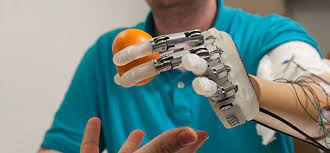
\includegraphics[height=0.4\textwidth,width=0.4\textwidth]{prothese.jpg}
    }
    \only<2>{
        \vspace{-10mm}
        \centering
        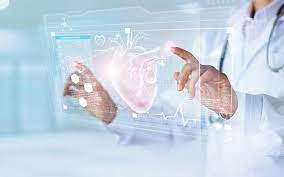
\includegraphics[height=0.4\textwidth,width=0.4\textwidth]{cardio.jpg}
    }
    \vspace{80mm}
\end{frame}

\begin{frame}{Les différentes rôles de IA}
    \begin{enumerate}[<+-|alert@+>]
        \myitem Diagnostique:
        \myitem Médecine prédictive
        \myitem Nouveaux médicaments
    \end{enumerate}
        \only<1>{
            % \vspace{-10mm}
            \begin{exampleblock} {Diagnostique:}
                la comparaison entre différentes modalités d'imagerie une
                échographie antérieure et un examen d'imagerie par résonance
                magnétique 
            \end{exampleblock}
        }
        \only<2>{
            \begin{exampleblock} {Médecine prédictive:}
                Prédire une lésion rénale 48 heures avant! C'est possible grâce à ``
                Deep Learning, grâce à une société d'intelligence artificielle qui
                a développé un algorithme capable de détecter des marqueurs
                biologiques annonciateurs des lésions rénales. ce qui permettrait de
                réduire de 11 \% les décès dus à ce genre d'événement. L'IA serait
                aussi capable de prédire la maladie d'Alzheimer en analysant des
                images cérébrales ou un échantillon sanguin, et même des accidents
                cardiaques en fonction d'un électrocardiogramme (ECG).
            \end{exampleblock}
        }
        \only<3>{
            \begin{exampleblock} {Nouveaux médicaments:}
                En passant au crible des milliards de molécules, l'intelligence
                artificielle est capable de prédire celles qui vont correspondre à un
                récepteur de cellule ou d'un virus. En juillet 2019, une équipe
                australienne a ainsi conçu le premier vaccin doté d'un adjuvant trouvé
                par un algorithme. L'IA permet d'élargir le champ des
                candidats-médicaments à des molécules que les chercheurs ne
                soupçonnaient pas, et de mieux anticiper les effets secondaires des
                futurs médicaments.\mybox
            \end{exampleblock}
        }
    \vspace{80mm}
\end{frame}


